%%%%%%%%%%%%%%%%%%%%%%%%%%%%%%%%%%%%%%%%%%%%%%%%%%%%%%%%%%%%%%%%%%%%%%%%%%%%%%%%%%%%%%%%%%%%%%%%%%%%%%%%%%%%%%%%%%%%%%%%%%%%%%%%%%%%%%%%%%%%%%%%%%%%%%%%%%%
% This is just an example/guide for you to refer to when submitting manuscripts to Frontiers, it is not mandatory to use Frontiers .cls files nor frontiers.tex  %
% This will only generate the Manuscript, the final article will be typeset by Frontiers after acceptance.   
%                                              %
%                                                                                                                                                         %
% When submitting your files, remember to upload this *tex file, the pdf generated with it, the *bib file (if bibliography is not within the *tex) and all the figures.
%%%%%%%%%%%%%%%%%%%%%%%%%%%%%%%%%%%%%%%%%%%%%%%%%%%%%%%%%%%%%%%%%%%%%%%%%%%%%%%%%%%%%%%%%%%%%%%%%%%%%%%%%%%%%%%%%%%%%%%%%%%%%%%%%%%%%%%%%%%%%%%%%%%%%%%%%%%

%%% Version 3.4 Generated 2022/06/14 %%%
%%% You will need to have the following packages installed: datetime, fmtcount, etoolbox, fcprefix, which are normally inlcuded in WinEdt. %%%
%%% In http://www.ctan.org/ you can find the packages and how to install them, if necessary. %%%
%%%  NB logo1.jpg is required in the path in order to correctly compile front page header %%%

\documentclass[utf8]{FrontiersinHarvard} % for articles in journals using the Harvard Referencing Style (Author-Date), for Frontiers Reference Styles by Journal: https://zendesk.frontiersin.org/hc/en-us/articles/360017860337-Frontiers-Reference-Styles-by-Journal
%\documentclass[utf8]{FrontiersinVancouver} % for articles in journals using the Vancouver Reference Style (Numbered), for Frontiers Reference Styles by Journal: https://zendesk.frontiersin.org/hc/en-us/articles/360017860337-Frontiers-Reference-Styles-by-Journal
%\documentclass[utf8]{frontiersinFPHY_FAMS} % Vancouver Reference Style (Numbered) for articles in the journals "Frontiers in Physics" and "Frontiers in Applied Mathematics and Statistics" 

%\setcitestyle{square} % for articles in the journals "Frontiers in Physics" and "Frontiers in Applied Mathematics and Statistics" 
\usepackage{url,hyperref,lineno,microtype,subcaption}
\usepackage{xcolor}
\usepackage[onehalfspacing]{setspace}
\usepackage{algorithm}
\usepackage{algorithmic}

\linenumbers


% Leave a blank line between paragraphs instead of using \\


\def\keyFont{\fontsize{8}{11}\helveticabold }
\def\firstAuthorLast{\textcolor{red}{Robalino-Díaz {et~al.}}} %use et al only if is more than 1 author
\def\Authors{Jorge Robalino-Díaz\,$^{1}$\textcolor{red}{,} Alejandro Cabrera-Andrade\,$^{2,3}$, Ana Karina Zambrano\,$^{4}$, and William Villegas-Ch\,$^{1*}$}
% Affiliations should be keyed to the author's name with superscript numbers and be listed as follows: Laboratory, Institute, Department, Organization, City, State abbreviation (USA, Canada, Australia), and Country (without detailed address information such as city zip codes or street names).
% If one of the authors has a change of address, list the new address below the correspondence details using a superscript symbol and use the same symbol to indicate the author in the author list.
\def\Address{$^{1}$Escuela de Ingeniería en Ciberseguridad, Facultad de Ingeniería y Ciencias Aplicadas, Universidad de Las Américas 170129, Quito, Ecuador\\ 
	$^{2}$Carrera de Enfermería, Facultad de Ciencias de la Salud, Universidad de las Américas, Quito 170125, Ecuador\\
	
	$^{3}$Grupo de Bio-Quimioinformática, Universidad de las Américas, Quito 170125, Ecuador 
	
	$^{4}$Universidad UTE, Facultad de Ciencias de la Salud Eugenio Espejo, Centro de Investigación Genética y Genómica, Quito 170129, Ecuador}
% The Corresponding Author should be marked with an asterisk
% Provide the exact contact address (this time including street name and city zip code) and email of the corresponding author
\def\corrAuthor{William Villegas-Ch}

\def\corrEmail{william.villegas@udla.edu.ec}




\begin{document}
\onecolumn
\firstpage{1}

\title[Running Title]{Multi-Environment Evaluation and Decision-Level Analysis of Clinical Prediction Models under Dataset Shift} 

\author[\firstAuthorLast ]{\Authors} %This field will be automatically populated
\address{} %This field will be automatically populated
\correspondance{} %This field will be automatically populated

\extraAuth{}% If there are more than 1 corresponding author, comment this line and uncomment the next one.
%\extraAuth{corresponding Author2 \\ Laboratory X2, Institute X2, Department X2, Organization X2, Street X2, City X2 , State XX2 (only USA, Canada and Australia), Zip Code2, X2 Country X2, email2@uni2.edu}


\maketitle


\begin{abstract}

%%% Leave the Abstract empty if your article does not require one, please see the Summary Table for full details.
\section{}
\textcolor{red}{Clinical machine-learning models are often evaluated within a single dataset, although deployment occurs across heterogeneous institutions and measurement processes. We evaluated Logistic Regression, Random Forest, and Gradient Boosting for ICU hospital-mortality prediction across MIMIC-III Demo and eICU using a revised primary specification based on a 24-hour landmark window and predictors observed in both domains. A decision-level diagnostic analysis examined how predicted-probability distributions interact with a fixed 0.5 threshold. Cross-domain discrimination was weak and often statistically compatible with chance-level performance. In eICU-to-MIMIC transfer, AUC-ROC was 0.523 for Logistic Regression, 0.583 for Random Forest, and 0.588 for Gradient Boosting. Random Forest generated no positive predictions, but this threshold failure was already present in internal eICU validation. Logistic Regression preserved sensitivity only through near-universal positive classification, whereas Gradient Boosting achieved limited detection. These findings show that clinical model evaluation should examine calibration, threshold behavior, and source-to-target operating-point stability, not only aggregate discrimination.}

\tiny
 \keyFont{ \section{Keywords:} Cross-domain clinical prediction, Dataset shift, Multi-environment Learning, Decision-level analysis, Probabilistic classification.} %All article types: you may provide up to 8 keywords; at least 5 are mandatory.
\end{abstract}

\section{Introduction}

The use of machine learning models in clinical prediction has grown steadily due to the availability of electronic health records (EHRs) and the ability of these records to capture complex relationships among physiological and biochemical variables. However, much of this development has been evaluated under the assumption of distributional homogeneity, in which training and test data come from the same clinical setting. This condition, while convenient from an experimental perspective, does not reflect the operational reality of healthcare systems, where models must be generalized to different populations, institutions, and protocols. Recent literature indicates that this discrepancy leads to \textcolor{red}{marked} performance degradation when models are deployed outside their original domain, particularly in critical tasks such as mortality prediction~\cite{Abdillah2024,Denada2025}.

The problem is exacerbated in multi-center settings, where heterogeneity between datasets such as MIMIC and eICU introduces differences in variable distribution, event prevalence, and data acquisition processes. These variations directly affect the structure of the models and their generalizability, a phenomenon known as dataset shift. Recent studies have addressed this phenomenon from the perspective of domain adaptation, proposing techniques to align representations across different data sources\citealp{Tayal2025}. However, these approaches often focus on improving overall metrics without explicitly analyzing how models make decisions under conditions of distributional misalignment. Additionally, research on feature selection has shown that the stability of selected variables can vary \textcolor{red}{substantially} across domains, affecting model consistency~\citet{Vlasic2025}.

A critical limitation in the evaluation of clinical models arises here: the use of aggregate metrics, such as accuracy or AUC-ROC, does not allow identification of structural flaws in model behavior, especially in detecting rare events. Recent work has indicated that interpretability and understanding of the decision-making process are fundamental for the adoption of models in clinical settings~\citet{Oh2024}, highlighting the need for approaches that go beyond average performance and analyze the relationship between predicted probabilities and final decisions. Furthermore, studies on medical classification have shown that class imbalance and overlap between distributions can \textcolor{red}{materially} affect model sensitivity, even when overall metrics suggest good performance~\citet{Ye2025}.

Based on these limitations, this work posits as its central problem the inability of traditional evaluation frameworks to capture the actual behavior of models under conditions of transfer between clinical domains. Specifically, the aim is to answer how the distribution of predicted probabilities changes when a model trained in one environment is evaluated in another, how this variation affects the application of a fixed decision threshold, and consequently, how the model's ability to detect the positive class is modified. This is integrated into \textcolor{red}{a decision-level diagnostic analysis} that enables interpretation of the model's behavior at the decision level, establishing an explicit connection between probabilistic estimation and the final class assignment.

To address this problem, a multi-environment evaluation protocol is proposed that integrates heterogeneous clinical datasets and defines explicit cross-domain transfer scenarios. This protocol is complemented by \textcolor{red}{a fixed-threshold decision diagnostic} focused on the probability distribution $f_{\theta}(x)$ and the application of an unchanged conventional decision threshold, allowing for the characterization of model behavior beyond aggregated metrics. \textcolor{red}{The primary methodology uses variables observed in both clinical domains and restricts feature construction to the first 24 hours after ICU admission. A full-episode/full-feature specification is reported separately as a retrospective sensitivity analysis.} The methodology includes constructing an integrated dataset from MIMIC and eICU, selecting comparable variables across domains, and evaluating representative models, such as Logistic Regression, Random Forest, and Gradient Boosting, under intra-domain and cross-domain conditions.

\textcolor{red}{The results show that, under the primary 24-hour shared-feature specification, all models have limited cross-domain transportability. In Train eICU $\rightarrow$ Test MIMIC, Random Forest produced no positive predictions at the fixed 0.5 threshold; however, this same threshold failure was already present during internal eICU validation, so it cannot be attributed exclusively to transfer. Gradient Boosting recovered only partial positive-class activation and Logistic Regression achieved high sensitivity at the cost of 89 false positives among 90 non-events.} These findings demonstrate that performance degradation is not only manifested in global metrics but also in the structure of the decision-making process itself, highlighting the importance of analyzing the relationship between the probability distribution and the classification threshold. This work contributes to the state of the art by \textcolor{red}{empirically characterizing fixed-threshold decision failure under clinical dataset shift, while distinguishing failures already present in the source domain from those amplified during transfer, rather than proposing probability-threshold analysis as a new mathematical construct,} and provides a methodological basis for developing more robust and reliable systems in real-world settings.

\section{Literature Review}

The development of clinical prediction models based on machine learning has evolved \textcolor{red}{rapidly} in recent years, driven by the availability of heterogeneous data from EHRs and distributed clinical systems. In this context, algorithms such as Logistic Regression, Random Forest, and boosting methods have demonstrated consistent performance in disease prediction tasks. However, their effectiveness depends largely on data quality, variable selection, and the specific conditions of the clinical environment~\citet{Abdillah2024}. Recent studies have shown that deep learning models can achieve higher levels of accuracy with complex data. Still, their performance remains conditioned by data distribution and the availability of representative information~\citet{Denada2025}.

One of the main challenges identified in the literature is the generalization of models in heterogeneous clinical settings, where the assumption of independence and identical distribution (i.i.d.) does not hold. This phenomenon, known as domain shift, has been widely documented in medical applications, where variations in equipment, clinical protocols, and population characteristics generate \textcolor{red}{material} differences between datasets~\citet{Matta2024}. In this regard, the analysis of distributional shifts has become a central focus of current research, highlighting the need to develop models that maintain their performance outside the training domain.

Empirical evidence demonstrates that clinical models experience \textcolor{red}{substantial} degradation when evaluated in populations not seen during training.~\citet{Musa2026} report that the performance of deep learning models can decrease by 10~\%--25~\% when applied across different populations, demonstrating the direct impact of domain shift on generalizability. This behavior is attributed to differences in disease prevalence, demographic characteristics, and data collection processes. Furthermore, mitigation strategies, such as domain adaptation and transfer learning, have been observed to offer limited improvements, with performance increases ranging from 5~\% to 15~\%, indicating that the problem is not fully resolved by conventional techniques.

In the realm of structured clinical data, integrating multiple information sources introduces an additional layer of complexity.~\citep{Chen2025} highlight that the coexistence of structured and unstructured data, along with heterogeneity across institutions, limits models' ability to learn cross-domain invariant representations. Additionally, data-driven studies, such as MIMIC, have demonstrated that the appropriate selection of variables is critical for maintaining model performance, especially when dimensionality is reduced without \textcolor{red}{substantially} affecting predictive capacity~\citet{Wang2025}.

The role of feature selection becomes more relevant in multi-domain scenarios, where the stability of the selected variables directly influences the model's robustness.~\citet{Theng2023} point out that the sensitivity of selection algorithms to data variations can affect the model's consistency across different environments. Along these lines, more recent approaches have incorporated advanced techniques, such as hybrid models and methods based on clinical knowledge, which improve interpretability and reduce data redundancy~\citet{Dardour2025,Sowan2025}.

Another relevant aspect in the literature is external and multicenter validation, which remains limited in many clinical studies.~\citet{Mercier2026} demonstrate that most models are validated using cross-validation schemes, whereas prospective or multicenter validation is less frequent, thereby limiting the models' real-world applicability. This problem is exacerbated by the lack of standardization in assessment metrics and the definition of clinical outcomes, which hinders comparisons between studies.

Finally, recent literature has begun to explore the relationship between prediction and explainability, highlighting the importance of understanding models' internal behavior in clinical settings.~\citet{Oh2024} points out that although predictive models are effective at identifying patterns, integrating them with interpretable approaches is essential for adoption in medical practice. This need becomes critical in scenarios where decisions depend not only on overall performance but also on the model's ability to respond consistently to data variations.


\section{Materials and Methods}
\subsection{Multi-source data acquisition and domain definition}

The study is built upon \textcolor{red}{two primary clinical data sources used for mortality prediction: MIMIC-III Clinical Database Demo v1.4, derived from the MIMIC-III critical care resource}~\citet{Johnson2016MIMIC,PhysioNetMIMICIIIDemo2019}, \textcolor{red}{and the eICU Collaborative Research Database}~\citet{Pollard2018eICU,PhysioNeteICU2018}. \textcolor{red}{After peer review, MedDialog was removed from the analytic scope of this manuscript because it has no hospital-mortality endpoint and no physiological feature space comparable with MIMIC or eICU.} The multi-environment configuration is defined from these sources using a source\_dataset variable and an environment type, thereby allowing distinction between intra-domain and cross-transfer scenarios during evaluation.

MIMIC serves as a reference for a single-center ICU environment, where clinical measurements (vital signs and laboratory tests) follow relatively consistent practices. eICU, on the other hand, integrates data from multiple hospitals and incorporates variability in protocols, instrumentation, and patient profiles. This difference is reflected in the construction of the integrated dataset, where both sources are combined while maintaining the source label, to enable two evaluation configurations: internal validation (training and testing within eICU) and cross-transfer (train eICU $\rightarrow$ test MIMIC and train MIMIC $\rightarrow$ test eICU). \textcolor{red}{The unit of analysis was the ICU episode: \texttt{icustay\_id} in MIMIC and \texttt{patientunitstayid} in eICU. The binary outcome was in-hospital mortality, operationalized as \texttt{hospital\_expire\_flag} in MIMIC and \texttt{actualhospitalmortality} in eICU after conversion to a binary label. Records without a resolvable mortality outcome were excluded from supervised modeling.}

The prediction target is defined as hospital mortality (\texttt{target\_mortality}), derived from the variables available in each clinical source. Integration is performed at the episode/admission level (\texttt{case\_id}), preserving the correspondence between records and the output label. This definition allows for direct comparison of model behavior under domain changes while maintaining task consistency.

The operational definition of the multi-domain environment is therefore determined by \textcolor{red}{the two clinical domains with different institutional origins (MIMIC vs.\ eICU), which are used for intra-domain evaluation and cross-transfer.}

\textcolor{red}{Cohort construction followed a deterministic episode-level procedure. MIMIC episodes were extracted from the demo critical-care tables by linking ICU stays to admissions and retaining episodes with an available \texttt{hospital\_expire\_flag}. eICU episodes were extracted using \texttt{patientunitstayid} as the episode identifier and retaining records with a non-missing \texttt{actualhospitalmortality}. The full-episode supervised cohort contained 136 MIMIC episodes and 3,676 eICU episodes. The primary 24-hour landmark cohort contained 124 MIMIC episodes and 2,438 eICU episodes after excluding episodes with identifiable death or discharge before completion of the 24-hour observation window. Because the MIMIC demo resource is intentionally small, this cohort should not be interpreted as representative of the full MIMIC population or of a general ICU population; it is used here as a constrained external-domain stress test. No patient-level clustering, repeated-admission exclusion beyond the available episode identifier, or hospital-level leave-site-out split was performed. These design choices are acknowledged as limitations when interpreting transfer performance.}

\subsection{Data preprocessing and feature construction}

Preprocessing is performed independently for each data source, maintaining traceability of each observation through a unique episode identifier (\texttt{case\_id}) and its source (\texttt{source\_dataset}). In structured clinical datasets (MIMIC and eICU), the variables correspond to time series of physiological and laboratory measurements recorded at different times throughout the patient's stay~\citet{Wan2025}. \textcolor{red}{The primary analysis uses a landmark design in which measurements are summarized only from the first 24 hours after ICU admission. The original full-episode construction is retained as a retrospective secondary analysis because it summarized all available episode measurements and can therefore include information recorded after a clinically plausible prediction time. This revision directly addresses the concern that full-stay aggregation could introduce temporal leakage.} Since the time length $T_i$ of each episode $i$ is variable, an aggregation process is applied that transforms these series into fixed-dimensional representations.

Let $x_{i,t}^{(j)}$ be the observed value of the clinical variable $j$ for case $i$ at time $t$, with $t \in \{1, \dots, T_i\}$. For each variable, statistical descriptors are constructed that capture both central tendency and intra-episode variability, including the mean (Equation~\ref{eq:mean_descriptor}), standard deviation (Equation~\ref{eq:std_descriptor}), and minimum/maximum values (Equation~\ref{eq:minmax_descriptor}):

\begin{equation}
	\mu_i^{(j)} = \frac{1}{T_i} \sum_{t=1}^{T_i} x_{i,t}^{(j)}
	\label{eq:mean_descriptor}
\end{equation}

\begin{equation}
	\sigma_i^{(j)} = \sqrt{\frac{1}{T_i} \sum_{t=1}^{T_i} \left(x_{i,t}^{(j)} - \mu_i^{(j)} \right)^2}
	\label{eq:std_descriptor}
\end{equation}

\begin{equation}
	x_{i,\min}^{(j)} = \min_{t} x_{i,t}^{(j)}, \quad
	x_{i,\max}^{(j)} = \max_{t} x_{i,t}^{(j)}
	\label{eq:minmax_descriptor}
\end{equation}

This set of transformations allows for condensation of the temporal information into a feature vector that preserves the basic dynamics of each variable, regardless of the series length, which is necessary for training supervised models in a homogeneous vector space.

The handling of missing values is addressed using a selection criterion based on the proportion of missing values for each variable. Let $m_j$ be the missing value rate of variable $j$ out of the total set of $N$ observations, as defined in Equation~\ref{eq:missing_rate}:

\begin{equation}
	m_j = \frac{1}{N} \sum_{i=1}^{N} \mathbb{I}\left(x_i^{(j)} = \text{NaN}\right)
	\label{eq:missing_rate}
\end{equation}

where $\mathbb{I}(\cdot)$ is the indicator function. A variable retention threshold is established such that $m_j \leq 0.60$, which ensures that each feature included in the model has sufficient statistical support. This filtering prevents the introduction of noise from variables with low completeness and stabilizes training on heterogeneous data.

Once the variables are selected, the features are organized in a common space that includes physiological descriptors observed in both MIMIC and eICU. \textcolor{red}{The primary 24-hour shared-feature model used 32 pre-encoding predictors: age, gender, and mean/minimum/maximum descriptors for ten clinical variable families: heart rate, temperature, respiratory rate, systolic blood pressure, diastolic blood pressure, glucose, creatinine, white blood cell count, sodium, and blood urea nitrogen. After preprocessing, gender was one-hot encoded inside the training pipeline, so the final model matrix could contain more columns than the clinical-variable count. Source-specific predictors were excluded from the primary transfer models, including \texttt{hospitalid}, \texttt{apachescore}, \texttt{predictedhospitalmortality}, and any variable completely absent in one domain. This is essential because \texttt{predictedhospitalmortality} is itself an APACHE-derived mortality estimate in eICU and would constitute a predictor derived for the same endpoint. The original 29-variable full-episode/full-feature model is therefore reported only as a retrospective secondary analysis and not as the primary evidence for cross-domain transportability.}

\subsection{Integrated dataset construction and labeling strategy}
The integrated dataset is constructed by combining clinical datasets from MIMIC and eICU, ensuring consistency across the feature space defined during preprocessing. Let $\mathcal{D}^{(M)}$ be the set of observations from MIMIC and $\mathcal{D}^{(E)}$ the corresponding set from eICU. The integrated dataset is defined as the union shown in Equation~\ref{eq:integrated_dataset}:

\begin{equation}
	\mathcal{D}^{(I)} = \mathcal{D}^{(M)} \cup \mathcal{D}^{(E)}
	\label{eq:integrated_dataset}
\end{equation}

where each observation $x_i \in \mathcal{D}^{(I)}$ belongs to a common feature space $\mathbb{R}^d$, previously aligned between both sources by selecting shared variables.

To preserve the traceability of the data's origin, a categorical origin variable $s_i$ is defined, which identifies the domain to which each observation belongs, as presented in Equation~\ref{eq:source_indicator}:

\begin{equation}
	s_i =
	\begin{cases}
		0, & \text{if } x_i \in \mathcal{D}^{(M)} \\
		1, & \text{if } x_i \in \mathcal{D}^{(E)}
	\end{cases}
	\label{eq:source_indicator}
\end{equation}

This variable allows for explicit distinction between data generation environments and forms the basis for defining intra-domain and cross-transfer evaluation scenarios.

The prediction target is defined as hospital mortality, represented by a binary variable $y_i \in \{0,1\}$, constructed from the indicators available in each source, as defined in Equation~\ref{eq:mortality_target}:

\begin{equation}
	y_i =
	\begin{cases}
		1, & \text{if the patient has mortality} \\
		0, & \text{otherwise}
	\end{cases}
	\label{eq:mortality_target}
\end{equation}

The integration of the datasets is performed under the condition of consistency in the definition of the target, so that all observations share the same output semantics, regardless of their origin.

Additionally, an environment characterization variable $e_i$ is introduced, which captures the differences in the data generation process, as presented in Equation~\ref{eq:environment_characterization}:

\begin{equation}
	e_i =
	\begin{cases}
		\text{single-center}, & \text{if } s_i = 0 \\
		\text{multi-center}, & \text{if } s_i = 1
	\end{cases}
	\label{eq:environment_characterization}
\end{equation}

This distinction enables the incorporation of relevant contextual information for analyzing model behavior, particularly in scenarios where cross-domain variability directly affects generalizability.

The process of building the integrated dataset follows a deterministic sequence that ensures feature alignment, label assignment, and the preservation of each observation's provenance. This procedure is formalized in Algorithm~\ref{alg:integrated_dataset_construction}.

\begin{algorithm}
	\caption{Integrated dataset construction for multi-environment learning}
	\label{alg:integrated_dataset_construction}
	
	\textbf{Input:}
	\begin{itemize}
		\item $D_M$: dataset from MIMIC
		\item $D_E$: dataset from eICU
	\end{itemize}
	
	\textbf{Output:}
	\begin{itemize}
		\item $D_I$: integrated dataset
	\end{itemize}
	
	\begin{algorithmic}[1]
		
		\STATE Align feature space between $D_M$ and $D_E$
		\STATE Initialize $D_I \leftarrow \emptyset$
		
		\FOR{each sample $x$ in $D_M$}
		\STATE assign \texttt{source\_dataset} $\leftarrow$ MIMIC
		\STATE assign \texttt{environment\_type} $\leftarrow$ single-center
		\STATE append $x$ to $D_I$
		\ENDFOR
		
		\FOR{each sample $x$ in $D_E$}
		\STATE assign \texttt{source\_dataset} $\leftarrow$ eICU
		\STATE assign \texttt{environment\_type} $\leftarrow$ multi-center
		\STATE append $x$ to $D_I$
		\ENDFOR
		
		\STATE ensure target variable $y$ is defined for all samples
		\STATE return $D_I$
		
	\end{algorithmic}
\end{algorithm}

This formulation allows for the explicit definition of a multi-domain environment in which observations share a common representation space but differ in their origin and the conditions under which they were generated.

\subsection{Multi-environment modeling and evaluation protocol}

The modeling process is defined on the integrated dataset
$\mathcal{D}^{(I)} = \{(x_i, y_i, s_i)\}_{i=1}^{N}$,
where each observation $x_i \in \mathbb{R}^d$ represents an aligned feature vector, $y_i \in \{0,1\}$ corresponds to the target mortality variable, and $s_i$ identifies the domain of origin. Three supervised models with different representational capabilities are used: Logistic Regression as a linear model, Random Forest as a decision-tree ensemble, and Gradient Boosting as a sequential additive model oriented toward error minimization.

Model estimation is based on the probabilistic prediction of the target variable, where each model defines a function $f_{\theta}(x_i) \in [0,1]$ that represents the estimated probability of mortality. The classification decision is obtained by applying a fixed threshold $\tau$, defined in Equation~\ref{eq:binary_decision}:

\begin{equation}
	\hat{y}_i = \mathbb{I}\big(f_{\theta}(x_i) \geq \tau\big)
	\label{eq:binary_decision}
\end{equation}

where $\tau = 0.5$ and $\mathbb{I}(\cdot)$ is the indicator function. \textcolor{red}{The value $\tau=0.5$ is used as a fixed conventional reference threshold to assess the behavior of an unchanged decision rule; it was not selected in the source validation data and is not presented as an optimized clinical threshold. Because Logistic Regression and Random Forest were trained with balanced class weights, their raw probability outputs should be interpreted as model scores on a probability scale rather than as automatically calibrated estimates of absolute deployment risk.} This formulation decouples the probabilistic estimation process from the binary decision, facilitating analysis of the model's behavior across different distributions.

The experimental protocol is organized into four scenarios that differ in the relationship between the training and test sets. In the internal validation scenario, the model is trained and evaluated solely on eICU data, allowing its behavior to be analyzed under consistent data-distribution conditions. In the integrated cross-validation scenario, the entire dataset $\mathcal{D}^{(I)}$ is used under a stratified five-fold cross-validation scheme, preserving the class proportions in each subset. In the transfer scenarios, the model is trained in one domain and evaluated in another, explicitly defining distributional misalignment conditions.

Evaluation in transfer scenarios is formalized as a cross-domain generalization problem, in which the training and test distributions differ. Let $P_E(x, y)$ be the distribution associated with eICU and $P_M(x, y)$ the one corresponding to MIMIC. The evaluation condition is established in Equation~\ref{eq:distribution_shift}:

\begin{equation}
	P_{\text{train}}(x, y) \neq P_{\text{test}}(x, y)
	\label{eq:distribution_shift}
\end{equation}

This inequality introduces a domain change that directly affects the model's generalization capacity, enabling analysis of its behavior under structural and distributional variations. \textcolor{red}{For the eICU internal-validation scenario, a stratified 75\%/25\% train-test split was used with \texttt{random\_state=42}. Integrated cross-validation used \texttt{StratifiedKFold(n\_splits=5, shuffle=True, random\_state=42)} across the combined MIMIC-eICU clinical dataset. This integrated cross-validation estimates performance when both domains are represented during resampling; it is not interpreted as external validation because observations from both sources contribute to the cross-validation process.}

The complete training and evaluation procedure is explicitly described in Algorithm~\ref{alg:modeling_evaluation_protocol}, which defines the sequence for scenario selection, model training, prediction generation, and metric calculation. \textcolor{red}{All preprocessing operations were implemented inside a scikit-learn pipeline fitted only on the training split or training fold. Numeric variables were imputed using the training-set median and standardized using the training-set mean and standard deviation. Categorical variables were imputed using the most frequent training-set category and one-hot encoded with unseen categories ignored at test time. Logistic Regression used \texttt{penalty=l2}, \texttt{C=1.0}, \texttt{max\_iter=2000}, \texttt{solver=liblinear}, \texttt{class\_weight=balanced}, and the default intercept setting. Random Forest used \texttt{n\_estimators=300}, \texttt{criterion=gini}, \texttt{max\_depth=None}, \texttt{min\_samples\_split=2}, \texttt{min\_samples\_leaf=1}, \texttt{max\_features=sqrt}, \texttt{bootstrap=True}, \texttt{class\_weight=balanced}, and \texttt{random\_state=42}. Gradient Boosting used \texttt{loss=log\_loss}, \texttt{learning\_rate=0.1}, \texttt{n\_estimators=100}, \texttt{subsample=1.0}, \texttt{criterion=friedman\_mse}, \texttt{min\_samples\_split=2}, \texttt{min\_samples\_leaf=1}, \texttt{max\_depth=3}, \texttt{max\_features=None}, \texttt{random\_state=42}, and no class weighting in the primary analysis. No hyperparameter search was performed. The analysis was run with Python 3.8.10, scikit-learn 1.3.2, pandas 2.0.3, and NumPy 1.24.3.} This algorithm \textcolor{red}{summarizes} the experimental process and establishes a direct correspondence between each evaluated configuration and its results.

\begin{algorithm}
	\caption{Multi-environment modeling and evaluation protocol}
	\label{alg:modeling_evaluation_protocol}
	
	\textbf{Input:}
	\begin{itemize}
		\item $D_I$: integrated dataset
		\item Models: \{Logistic, RF, GB\}
	\end{itemize}
	
	\textbf{Output:}
	\begin{itemize}
		\item Performance metrics per scenario
	\end{itemize}
	
	\begin{algorithmic}[1]
		
		\STATE Define scenarios:
		\STATE \hspace{0.5cm} $S_1$: \texttt{eICU\_internal\_validation}
		\STATE \hspace{0.5cm} $S_2$: \texttt{integrated\_5fold\_cv}
		\STATE \hspace{0.5cm} $S_3$: \texttt{train\_eICU\_test\_MIMIC}
		\STATE \hspace{0.5cm} $S_4$: \texttt{train\_MIMIC\_test\_eICU}
		
		\FOR{each model in Models}
		\FOR{each scenario in $\{S_1, S_2, S_3, S_4\}$}
		\STATE Split data according to scenario definition
		\STATE Train model on training set
		\STATE Predict probabilities on test set
		\STATE Apply decision threshold $\tau = 0.5$
		\STATE Compute TP, TN, FP, FN
		\STATE Calculate metrics (Accuracy, Precision, Recall, F1, AUC)
		\ENDFOR
		\ENDFOR
		
		\STATE return results
		
	\end{algorithmic}
\end{algorithm}

Performance evaluation is based on the confusion matrix, considering the counts of true positives (TP), true negatives (TN), false positives (FP), and false negatives (FN). From these values, the evaluation metrics are defined through Precision (Equation~\ref{eq:precision_metric}), Recall (Equation~\ref{eq:recall_metric}), and F1-score (Equation~\ref{eq:f1_metric}):

\begin{equation}
	\text{Precision} =
	\frac{TP}{TP + FP}
	\label{eq:precision_metric}
\end{equation}

\begin{equation}
	\text{Recall} =
	\frac{TP}{TP + FN}
	\label{eq:recall_metric}
\end{equation}

\begin{equation}
	F1 =
	2 \cdot
	\frac{\text{Precision} \cdot \text{Recall}}
	{\text{Precision} + \text{Recall}}
	\label{eq:f1_metric}
\end{equation}

Additionally, the area under the ROC curve (AUC-ROC) is used as a measure of discriminative capacity independent of the decision threshold, allowing evaluation of class separability across different operating points.

\textcolor{red}{Because the reviewers specifically raised concerns about calibration and threshold selection, we added additional transfer analyses beyond the primary fixed-threshold results. Calibration was summarized using the Brier score, five-bin calibration gaps, expected calibration error, and post hoc calibration intercept and slope from a logistic recalibration model of the observed outcome on the logit of the predicted probability. We also computed average precision as a precision-recall summary for imbalanced outcomes. Finally, we evaluated post hoc F1-maximizing thresholds on the test predictions only as a sensitivity analysis. These optimized thresholds are not proposed as deployable clinical cutoffs because they use test-set outcome information; they are included only to determine whether failure at $\tau=0.5$ reflects complete absence of ranking information or misalignment of the fixed conventional decision threshold. A fully deployable threshold-transportability experiment would require selecting the threshold exclusively within a source-domain validation set, locking it, and then applying it unchanged to the target domain.}

\textcolor{red}{A strict shared-feature specification was used as the primary analysis to address imperfect variable equivalence. In this analysis, all predictors that were completely absent in either source were excluded, including eICU-specific identifiers and severity-score variables (\texttt{hospitalid}, \texttt{apachescore}, and \texttt{predictedhospitalmortality}) and pressure-summary variables without equivalent cross-domain extraction. The resulting full-episode sensitivity predictor set contained age, gender, and shared heart-rate, respiratory-rate, glucose, creatinine, white-blood-cell, sodium, and blood-urea-nitrogen summary variables. The 24-hour primary predictor set used the corresponding early-window shared variables listed above.}

\textcolor{red}{Class imbalance was handled explicitly for Logistic Regression and Random Forest through balanced class weights, whereas Gradient Boosting was evaluated unweighted in the primary analysis because this estimator does not use a \texttt{class\_weight} parameter. To assess whether this modeling choice explained the transfer failure, we added a sensitivity analysis comparing weighted and unweighted variants. In Train eICU $\rightarrow$ Test MIMIC, unweighted Random Forest still generated no positive predictions, and inverse-frequency sample weighting for Gradient Boosting recovered only two true positives (recall 0.043, F1-score 0.078). Thus, class weighting changed the operating point of some models but did not remove the cross-domain fixed-threshold failure.}

The structure of the multi-environment evaluation protocol, including dataset integration, internal validation, and cross-transfer scenarios, is presented in Figure~\ref{fig:fig1}, which illustrates the relationships between domains, training and testing paths, and the configurations used in each experimental scenario.

\begin{figure}[h!]
	\begin{center}
		\includegraphics[width=16cm]{Fig1.jpg}% This is a *.eps file
	\end{center}
	\caption{Multi-environment modeling and evaluation protocol for cross-domain clinical prediction.}\label{fig:fig1}
\end{figure}

\subsubsection{\textcolor{red}{Decision-level diagnostic analysis for cross-domain transfer}}
The analysis of the model's behavior is framed at the decision level, focusing on the transformation of predicted probabilities into binary outputs using a fixed threshold. Let $f_{\theta}(x_i) \in [0,1]$ be the estimated probability of the positive class for an observation $x_i$. The decision rule is defined by applying a fixed threshold $\tau = 0.5$ to the predicted probabilities, yielding a binary output $\hat{y}_i \in \{0,1\}$.

This formulation decouples the probabilistic estimation process from the decision mechanism, establishing \textcolor{red}{a diagnostic strategy} to study how the shape of the probability distribution influences the final class assignment.

The \textcolor{red}{diagnostic approach} is based on analyzing the conditional distribution of $f_{\theta}(x)$ given the true class $y$, which allows evaluation of the separability between classes in the probability space. For each evaluation scenario, the predicted probabilities are grouped by the actual label $y$, enabling characterization of the degree of overlap, concentration, and displacement of the probability mass. This characterization defines the conditions under which the threshold-induced transformation can generate consistent decisions or \textcolor{red}{become unstable across domains}.

The application of the threshold $\tau$ induces a partitioning of the decision space whose stability depends directly on the structure of the probability distribution. In the presence of well-separated distributions, the threshold produces balanced assignments between the classes. In contrast, when the probabilities are concentrated in specific regions or exhibit \textcolor{red}{substantial} overlap, the resulting assignment may show dominance of one class, thereby affecting the model's ability to discriminate adequately between positive and negative events.

The structural representation of this process is shown in Figure~\ref{fig:fig2}, which formalizes the sequence of transformations from the model input to the final decision. The scheme explicitly distinguishes between conditions of distributional alignment and misalignment between domains and establishes differentiated trajectories in the decision-making process. This formulation allows the model's behavior to be interpreted as a function of the relationship between the probabilistic estimate and the decision threshold, regardless of the specific evaluation scenario.

\begin{figure}[h!]
	\begin{center}
		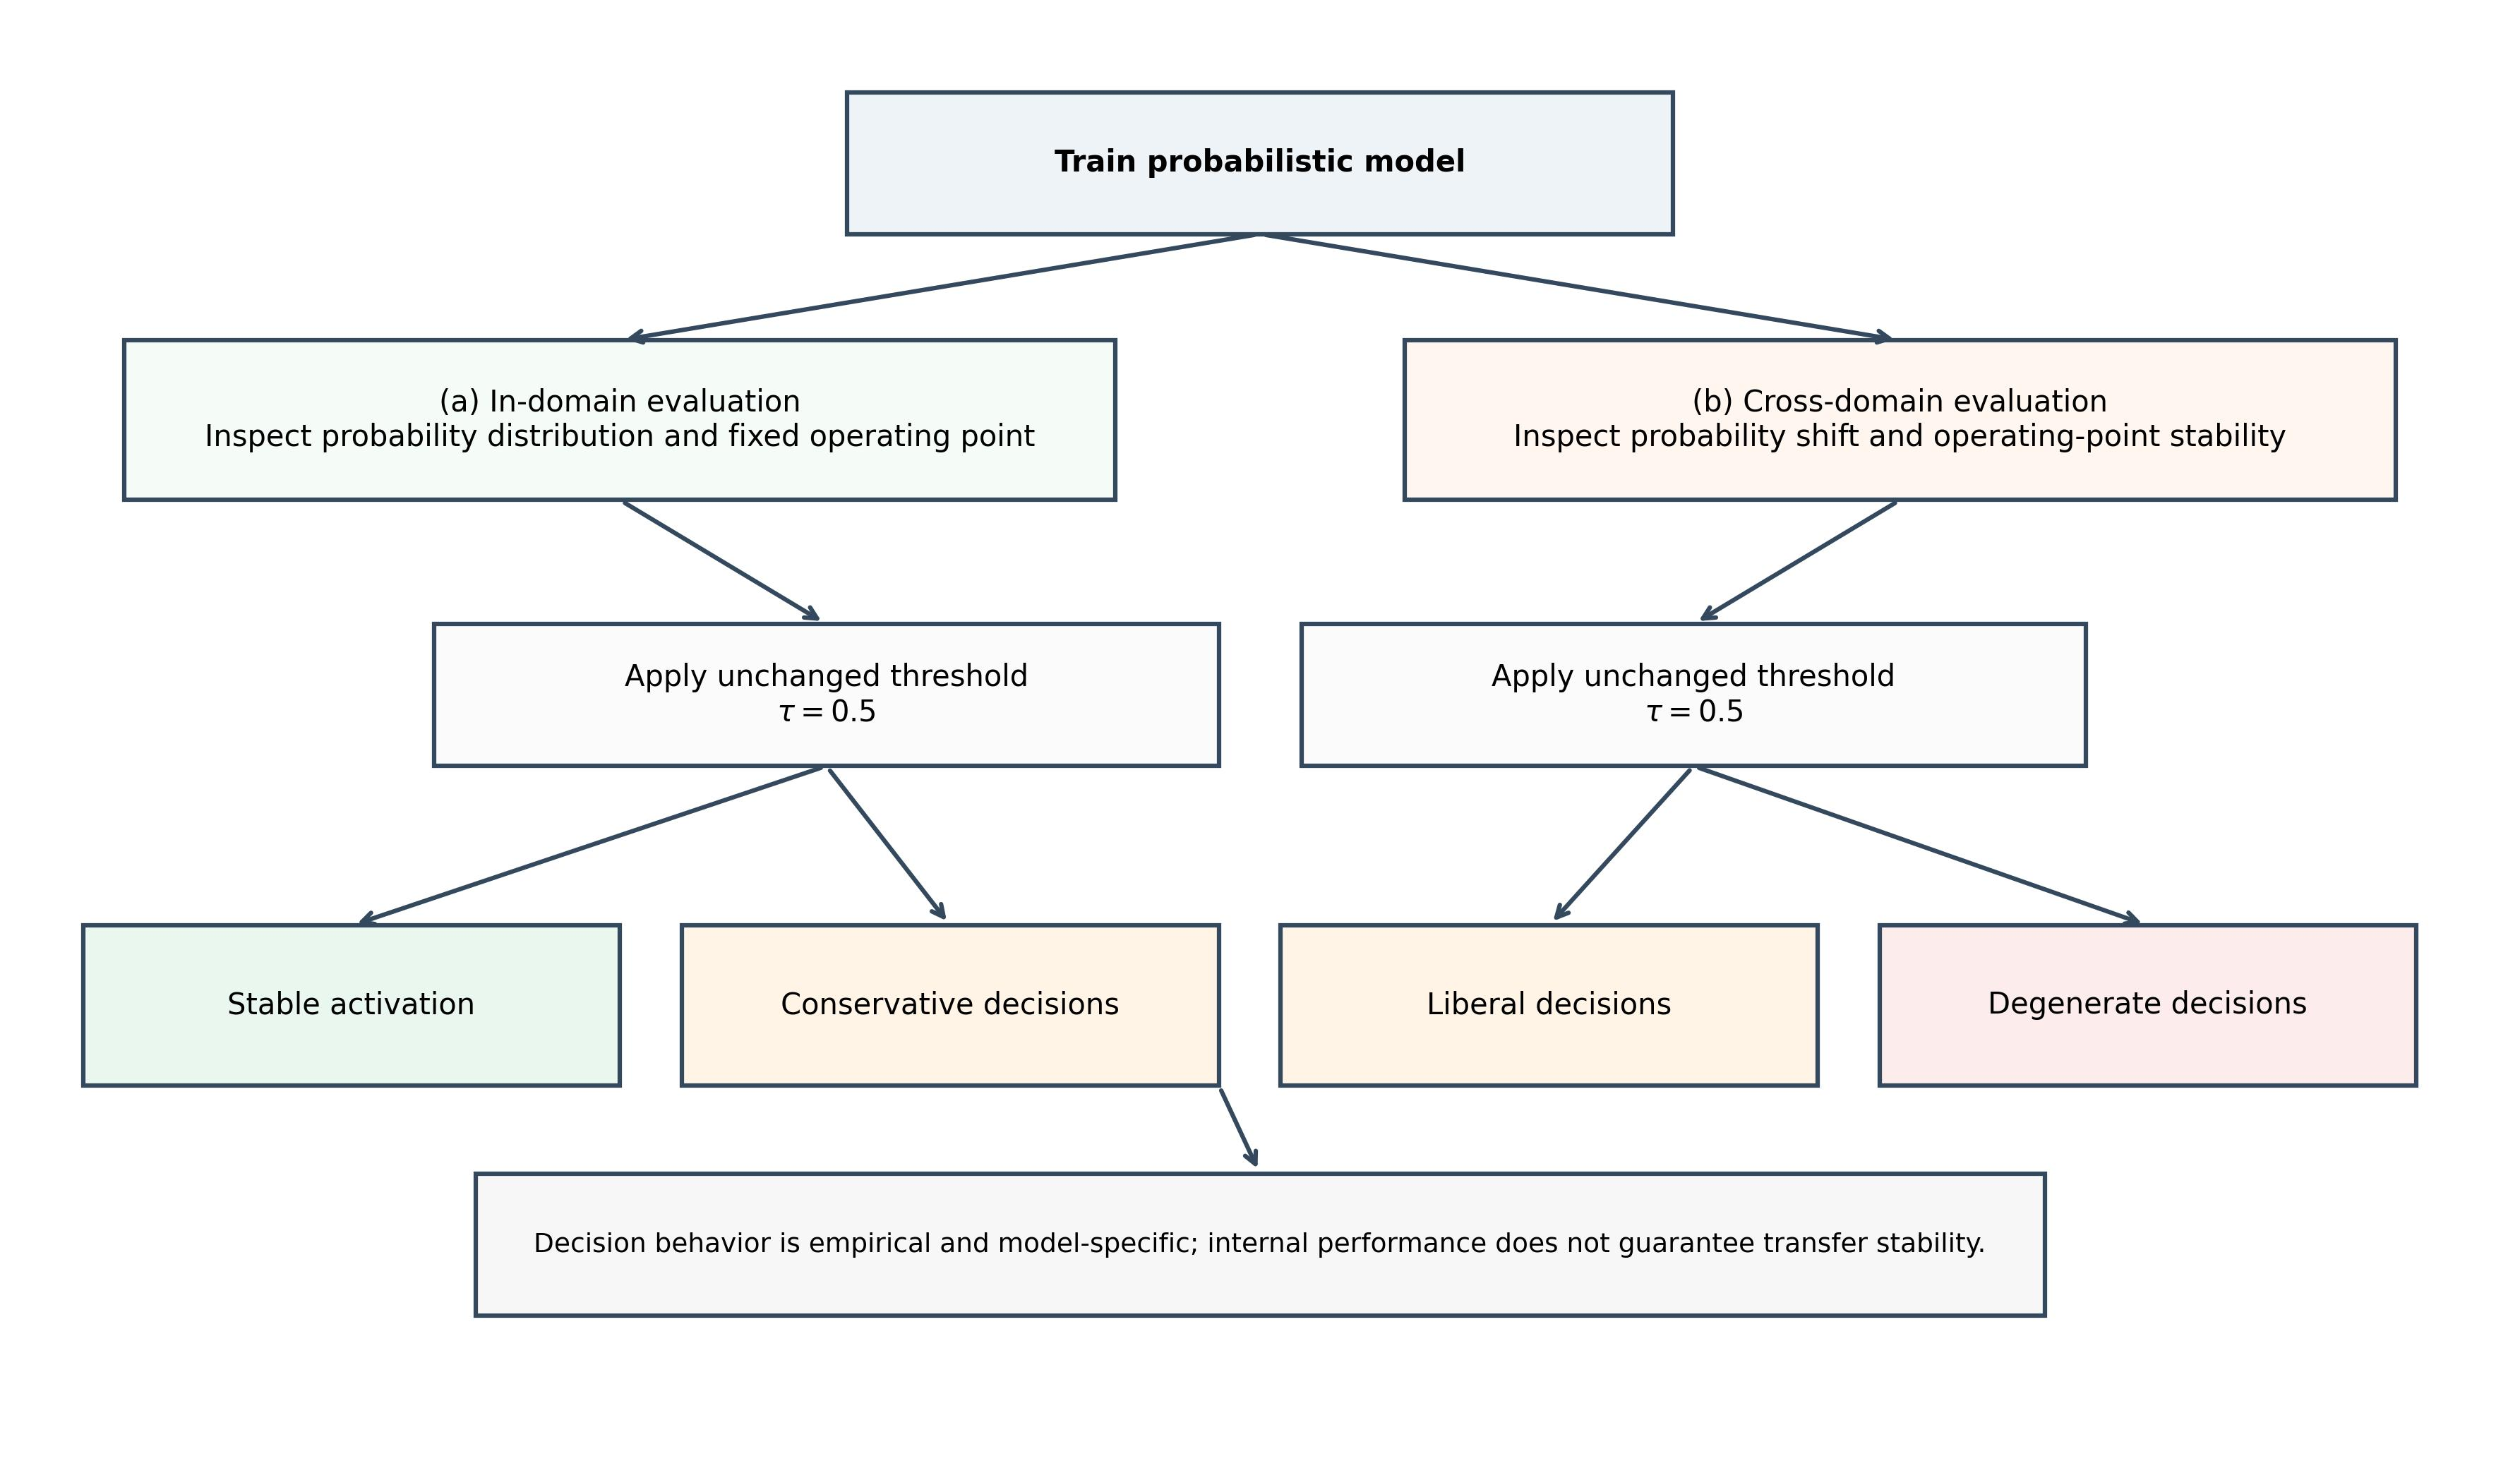
\includegraphics[width=15cm]{Fig2.jpg}% This is a *.eps file
	\end{center}
	\caption{Decision-level behavior analysis under cross-domain conditions.}\label{fig:fig2}
\end{figure}

The \textcolor{red}{decision-level diagnostic analysis} is applied consistently across all scenarios defined in the experimental protocol, allowing us to study how variations in the probability distribution translate into changes in classification behavior at the decision level.

\section{Results}
\subsection{Characterization of the integrated dataset and selection of variables}
The composition of the integrated dataset reveals a marked asymmetry between the sources. The original dataset is dominated by eICU, with 4,358 records, compared to 136 in MIMIC, representing a difference of more than one order of magnitude. This relationship persists after cleaning, with the clean dataset containing 3,812 valid instances, thereby preserving eICU's dominance as the primary source of information.

Regarding the target variable, the class distribution shows notable differences between the datasets. In MIMIC, the 46 mortality events versus 90 non-mortality cases reflect a relatively balanced proportion (33.8~\% mortality). In contrast, in eICU, the ratio is \textcolor{red}{more unequal}, with 310 mortality events versus 3,366 non-mortality cases, corresponding to approximately 8.4~\% mortality. This divergence introduces a structural difference in the target distribution between the two environments, with MIMIC exhibiting a higher density of adverse events than eICU.

Analysis of the clean integrated dataset shows that this discrepancy translates into a pronounced overall imbalance, with 3,456 non-mortality cases versus 356 mortality events, corresponding to a ratio of approximately 90.7~\% to 9.3~\%. This configuration implies that the minority class is \textcolor{red}{underrepresented}, which limits the models' ability to capture patterns associated with critical events.

Additionally, it is observed that all 682 records without a target variable are concentrated in eICU, while MIMIC does not present any missing values in this dimension. Removing these records reduces the eICU volume to 3,676 valid instances, without substantially altering the class ratio in this source. \textcolor{red}{Because outcome-missingness is source-specific, we do not assume that these exclusions are fully non-informative; rather, we report their concentration in eICU and interpret the resulting cohort as the analyzable supervised subset.}

Table~\ref{table:integrated_dataset_structure} presents the consolidated dataset structure for the original full-episode matrix, including the number of records per source before and after cleaning, the class distribution, and the number of retained variables (29). This representation allows simultaneous observation of the scale difference between the datasets, the concentration of missing values, and the final configuration of the dataset used in the secondary retrospective analysis.

\begin{table}[h]
	\caption{Dataset composition and class distribution across MIMIC, eICU, and integrated clinical dataset}
	\label{table:integrated_dataset_structure}
	\setlength{\tabcolsep}{3pt}
	\begin{tabular}{p{125pt}p{55pt}p{55pt}p{140pt}}
		\hline
		\textbf{Metric} & \textbf{MIMIC} & \textbf{eICU} & \textbf{Integrated clean dataset} \\ \hline
		Raw samples & 136 & 4358 & 4494 \\
		Valid samples & 136 & 3676 & 3812 \\
		Non-mortality cases & 90 & 3366 & 3456 \\
		Mortality cases & 46 & 310 & 356 \\
		Missing target & 0 & 682 & 682 \\
		Retained variables & 29 & 29 & 29 \\
		Mortality proportion & 33.8~\% & 8.4~\% & 9.3~\% \\ \hline
	\end{tabular}
	\footnotesize
\end{table}

Regarding variable completeness, the missing values analysis indicates that central tendency metrics show relatively low levels of missingness. Variables such as \texttt{hr\_mean}, \texttt{glucose\_mean}, and \texttt{bun\_mean} show missing percentages of less than 3~\%, while derived variables such as \texttt{wbc\_std}, \texttt{bun\_std}, and \texttt{creatinine\_std} reach levels close to 10~\%--15~\%. This difference indicates that primary information associated with mean values is better represented than dispersion metrics, suggesting greater stability in capturing central tendency than in capturing intra-patient variability.

\textcolor{red}{The primary retained variable set no longer assumes that a 29-column structural matrix is equivalent to clinical harmonization. Instead, the primary 24-hour model uses 32 pre-encoding predictors derived from 10 shared clinical variable families plus age and gender. The original 29-variable full-episode matrix is described as a secondary retrospective specification. The strict full-episode shared-feature sensitivity model used 16 pre-encoding predictors, corresponding to age, gender, and mean/standard-deviation summaries for seven shared clinical variable families. In these matrices, completeness was not identical across sources: \texttt{hospitalid}, \texttt{apachescore}, \texttt{predictedhospitalmortality}, and some pressure summaries were not equivalent across MIMIC and eICU. Conversely, core vital-sign and laboratory summaries were present in both sources with low-to-moderate missingness. This pattern indicates that structural column alignment alone is insufficient as evidence of measurement equivalence.}

\subsection{Comparison of distributions between clinical settings}
The comparison of clinical variable distributions reveals consistent differences between the MIMIC and eICU datasets in both location and dispersion. For heart rate, both sources exhibit unimodal distributions with a high degree of overlap in the central range; however, a slight shift toward higher values is observed in MIMIC, with its maximum density concentrated around values slightly higher than those observed in eICU. Furthermore, the MIMIC distribution shows a longer right tail, indicating greater variability toward higher values than that of eICU.

Figure~\ref{fig:fig3}(a) presents the comparative distributions of the selected clinical variables in both environments. In Figure~\ref{fig:fig3}(a), which shows heart rate, both distributions have a similar shape, with an approximately unimodal pattern. However, the MIMIC curve shows a slight shift toward higher values, with greater density in the 85--100 range. eICU, on the other hand, shows a higher concentration in the slightly lower ranges, with a steeper slope of decline following the peak. The overlap between the two curves is high in the mid-range but gradually decreases toward the extreme values, where MIMIC exhibits a longer tail.

\begin{figure}[h!]
	\begin{center}
		\includegraphics[width=17cm]{Fig3.jpg}% This is a *.eps file
	\end{center}
\caption{\textcolor{red}{Distribution of key primary shared clinical variables across datasets. (a) Heart rate distribution for MIMIC and eICU in beats per minute. (b) Glucose level distribution for MIMIC and eICU in mg/dL. (c) Creatinine distribution for MIMIC and eICU in mg/dL. (d) Systolic blood pressure distribution in mmHg. Kernel-density curves were generated from available non-missing values using the plotting library's default Gaussian kernel bandwidth.}}\label{fig:fig3}
\end{figure}

In Figure~\ref{fig:fig3}(b), corresponding to glucose levels, the differences between the datasets are more pronounced. eICU shows a more concentrated distribution, with a sharper peak around 110, followed by a rapid drop in density. In contrast, MIMIC shows a broader distribution, with a lower concentration at the peak and a considerable extension toward higher values. The right tail in MIMIC extends \textcolor{red}{well} beyond 250, while in eICU, the density decreases more abruptly, indicating greater dispersion in MIMIC.

In Figure~\ref{fig:fig3}(c), associated with creatinine, a structural difference in the shape of the distributions is observed. eICU shows a high density of values close to zero, with a pronounced peak and a rapid decline. In contrast, MIMIC exhibits a flatter distribution, with lower density at the minimum values and a greater extension toward the upper values. The MIMIC curve maintains a sustained presence over a broader range, reflecting greater variability compared to the strong concentration observed in eICU.

\textcolor{red}{Figure~\ref{fig:fig3}(d), corresponding to systolic blood pressure, replaces the previous mean-arterial-pressure panel so that all displayed variables are part of the primary shared-feature specification. The distributions overlap in the central range but differ in spread and tail behavior, reinforcing that nominally shared variables may still have different empirical distributions across source systems.}

\subsection{\textcolor{red}{Primary 24-hour shared-feature performance}}

\textcolor{red}{The primary analysis used the 24-hour landmark cohort and only predictors observed in both MIMIC and eICU. This specification was prioritized over the original full-episode/full-feature analysis because it reduces temporal leakage risk and avoids eICU-specific predictors such as \texttt{predictedhospitalmortality}, \texttt{apachescore}, and \texttt{hospitalid}. The performance of the models under intra-environment conditions is presented in Table~\ref{tab:intra_environment_performance}, considering both internal validation on eICU and integrated cross-validation.}

\begin{table}[h]
	\caption{\textcolor{red}{Primary 24-hour shared-feature intra-domain performance under internal validation and integrated cross-validation scenarios}}
	\label{tab:intra_environment_performance}
	\setlength{\tabcolsep}{3pt}
	\begin{tabular}{p{115pt}p{95pt}p{50pt}p{50pt}p{45pt}p{45pt}p{60pt}}
		\hline
		\textbf{Scenario} & \textbf{Model} & \textbf{Accuracy} & \textbf{Precision} & \textbf{Recall} & \textbf{F1-score} & \textbf{AUC-ROC} \\ \hline
		
		\textcolor{red}{eICU internal validation} & \textcolor{red}{LogisticRegression} & \textcolor{red}{0.718} & \textcolor{red}{0.145} & \textcolor{red}{0.675} & \textcolor{red}{0.239} & \textcolor{red}{0.778} \\
		\textcolor{red}{eICU internal validation} & \textcolor{red}{RandomForest} & \textcolor{red}{0.934} & \textcolor{red}{NA} & \textcolor{red}{0.000} & \textcolor{red}{0.000} & \textcolor{red}{0.740} \\
		\textcolor{red}{eICU internal validation} & \textcolor{red}{GradientBoosting} & \textcolor{red}{0.923} & \textcolor{red}{0.182} & \textcolor{red}{0.050} & \textcolor{red}{0.078} & \textcolor{red}{0.776} \\
		
		\textcolor{red}{Integrated 5-fold CV} & \textcolor{red}{LogisticRegression} & \textcolor{red}{$0.737 \pm 0.009$} & \textcolor{red}{$0.171 \pm 0.012$} & \textcolor{red}{$0.651 \pm 0.048$} & \textcolor{red}{$0.270 \pm 0.019$} & \textcolor{red}{$0.763 \pm 0.025$} \\
		
		\textcolor{red}{Integrated 5-fold CV} & \textcolor{red}{RandomForest} & \textcolor{red}{$0.925 \pm 0.002$} & \textcolor{red}{$0.200 \pm 0.400$} & \textcolor{red}{$0.010 \pm 0.021$} & \textcolor{red}{$0.020 \pm 0.039$} & \textcolor{red}{$0.771 \pm 0.024$} \\
		
		\textcolor{red}{Integrated 5-fold CV} & \textcolor{red}{GradientBoosting} & \textcolor{red}{$0.915 \pm 0.009$} & \textcolor{red}{$0.271 \pm 0.180$} & \textcolor{red}{$0.088 \pm 0.061$} & \textcolor{red}{$0.128 \pm 0.082$} & \textcolor{red}{$0.754 \pm 0.032$} \\ \hline
		
	\end{tabular}
	\footnotesize
\end{table}

\textcolor{red}{In the primary 24-hour shared-feature internal validation scenario on eICU, apparent performance was much more modest than in the original full-episode analysis. Logistic Regression produced the highest recall (0.675) but low precision (0.145), indicating many false-positive activations. Random Forest achieved high accuracy (0.934) and moderate AUC-ROC (0.740), but generated no positive predictions at the fixed 0.5 threshold; precision is therefore reported as NA rather than zero because TP+FP=0. Gradient Boosting showed similar discrimination (AUC-ROC 0.776) but very low recall (0.050).}

\textcolor{red}{In integrated five-fold cross-validation, AUC-ROC values remained in the range 0.754--0.771, but threshold-dependent minority-class metrics were weak for tree-based models. Random Forest had recall $0.010 \pm 0.021$ and F1-score $0.020 \pm 0.039$, while Gradient Boosting had recall $0.088 \pm 0.061$ and F1-score $0.128 \pm 0.082$. Logistic Regression again favored sensitivity over precision, with recall $0.651 \pm 0.048$ and precision $0.171 \pm 0.012$. These values indicate that the clinically stricter landmark/shared-feature design substantially reduces the apparent performance observed in the original full-episode/full-feature results.}

\textcolor{red}{The comparison between internal eICU validation and integrated cross-validation shows that tree-based models retain moderate rank-ordering ability when the evaluation structure allows both domains to contribute to the resampling process. However, this pattern should not be interpreted as evidence of external transportability, because integrated cross-validation still differs from strict train-on-one-domain/test-on-another-domain transfer. Random Forest is especially important: under the primary specification, the fixed 0.5 threshold was already unsuitable in internal eICU validation and remained unsuitable after transfer to MIMIC. Therefore, the absence of positive predictions in MIMIC cannot be attributed exclusively to cross-domain transfer.} Furthermore, the standard deviations observed in cross-validation are low across all metrics, particularly for accuracy and AUC-ROC, indicating consistent model performance \textcolor{red}{under mixed-domain resampling}.

\subsection{Multi-environment evaluation (transfer)}
\textcolor{red}{The performance of the models in cross-environment transfer scenarios is presented in Table~\ref{tab:cross_environment_transfer} for the primary 24-hour shared-feature specification. In the Train eICU $\rightarrow$ Test MIMIC scenario, cross-domain discrimination approached random-to-weak performance for all models, with AUC-ROC values between 0.523 and 0.588. Threshold-dependent behavior differed substantially across algorithms. Logistic Regression classified nearly all MIMIC test cases as positive, yielding high recall (0.971) but extremely low specificity (0.011) and accuracy (0.274). Random Forest generated no positive predictions at $\tau=0.5$, making precision undefined and producing recall and F1-score values of 0.000. Gradient Boosting recovered limited positive-class activation, with 8 true positives, 8 false positives, recall 0.235, and F1-score 0.320.}

\begin{table}[h]
	\caption{\textcolor{red}{Primary 24-hour shared-feature cross-domain model performance under transfer scenarios}}
	\label{tab:cross_environment_transfer}
	\setlength{\tabcolsep}{3pt}
	\begin{tabular}{p{140pt}p{50pt}p{50pt}p{50pt}p{45pt}p{45pt}p{60pt}}
		\hline
		\textbf{Scenario} & \textbf{Model} & \textbf{Accuracy} & \textbf{Precision} & \textbf{Recall} & \textbf{F1-score} & \textbf{AUC-ROC} \\ \hline
		
		\textcolor{red}{Train eICU $\rightarrow$ Test MIMIC} & \textcolor{red}{Logistic} & \textcolor{red}{0.274} & \textcolor{red}{0.270} & \textcolor{red}{0.971} & \textcolor{red}{0.423} & \textcolor{red}{0.523} \\
		\textcolor{red}{Train eICU $\rightarrow$ Test MIMIC} & \textcolor{red}{RF} & \textcolor{red}{0.726} & \textcolor{red}{NA} & \textcolor{red}{0.000} & \textcolor{red}{0.000} & \textcolor{red}{0.583} \\
		\textcolor{red}{Train eICU $\rightarrow$ Test MIMIC} & \textcolor{red}{GB} & \textcolor{red}{0.726} & \textcolor{red}{0.500} & \textcolor{red}{0.235} & \textcolor{red}{0.320} & \textcolor{red}{0.588} \\
		
		\textcolor{red}{Train MIMIC $\rightarrow$ Test eICU} & \textcolor{red}{Logistic} & \textcolor{red}{0.528} & \textcolor{red}{0.074} & \textcolor{red}{0.544} & \textcolor{red}{0.130} & \textcolor{red}{0.548} \\
		\textcolor{red}{Train MIMIC $\rightarrow$ Test eICU} & \textcolor{red}{RF} & \textcolor{red}{0.921} & \textcolor{red}{0.053} & \textcolor{red}{0.013} & \textcolor{red}{0.020} & \textcolor{red}{0.558} \\
		\textcolor{red}{Train MIMIC $\rightarrow$ Test eICU} & \textcolor{red}{GB} & \textcolor{red}{0.813} & \textcolor{red}{0.091} & \textcolor{red}{0.209} & \textcolor{red}{0.127} & \textcolor{red}{0.574} \\ \hline
		
	\end{tabular}
	\footnotesize
\end{table}

\textcolor{red}{In the reverse scenario, from Train MIMIC $\rightarrow$ Test eICU, no model achieved clinically strong positive-class detection. Logistic Regression again favored sensitivity over specificity, whereas Random Forest preserved high specificity (0.984) but detected only 2 of 158 deaths. Gradient Boosting detected 33 of 158 deaths but still had low precision (0.091) and F1-score (0.127). The comparison between directions therefore supports a narrower interpretation than the original submission: the central issue is weak transportable discrimination combined with instability of the probability scale and fixed-threshold decision rule.}

\textcolor{red}{To quantify uncertainty in the primary transfer results, we added stratified non-parametric bootstrap confidence intervals using 2,000 resamples within each test set. Bootstrap resamples preserved the observed event/non-event counts; no resamples were discarded for containing a single class. Sensitivity and specificity intervals were calculated using exact binomial confidence intervals because these quantities are conditional on the number of observed events or non-events and because a test-set bootstrap can otherwise produce misleading zero-width intervals when a model makes no positive predictions. Precision is reported as NA when TP+FP=0. In the Train eICU $\rightarrow$ Test MIMIC scenario, Random Forest had sensitivity 0.000 (95\% exact CI 0.000--0.103), specificity 1.000 (95\% exact CI 0.960--1.000), F1-score 0.000 (bootstrap CI 0.000--0.000), and AUC-ROC 0.583 (bootstrap CI 0.462--0.697). Gradient Boosting had sensitivity 0.235 (95\% exact CI 0.107--0.412), specificity 0.911 (95\% exact CI 0.832--0.961), F1-score 0.320 (bootstrap CI 0.157--0.490), and AUC-ROC 0.588 (bootstrap CI 0.469--0.711). Logistic Regression had sensitivity 0.971 (95\% exact CI 0.847--0.999) but specificity 0.011 (95\% exact CI 0.000--0.060), confirming that its high sensitivity was achieved by near-universal positive classification rather than clinically useful separation. These uncertainty results are summarized in Table~\ref{tab:transfer_uncertainty}.}

\begin{table}[h]
	\caption{\textcolor{red}{Uncertainty summary for primary 24-hour shared-feature cross-domain transfer results. E2M denotes Train eICU $\rightarrow$ Test MIMIC; M2E denotes Train MIMIC $\rightarrow$ Test eICU. Sensitivity and specificity intervals are exact binomial 95\% confidence intervals; accuracy, F1-score, AUC-ROC, and Brier intervals are stratified bootstrap 95\% intervals from 2,000 resamples. Precision is reported as NA when TP+FP=0.}}
	\label{tab:transfer_uncertainty}
	\setlength{\tabcolsep}{3pt}
	\tiny
	\resizebox{\textwidth}{!}{%
	\begin{tabular}{llllllll}
		\hline
		\textbf{\textcolor{red}{Scen.}} & \textbf{\textcolor{red}{Model}} & \textbf{\textcolor{red}{Precision}} & \textbf{\textcolor{red}{Sensitivity}} & \textbf{\textcolor{red}{Specificity}} & \textbf{\textcolor{red}{F1-score}} & \textbf{\textcolor{red}{AUC-ROC}} & \textbf{\textcolor{red}{Brier}} \\ \hline
		\textcolor{red}{E2M} & \textcolor{red}{LR} & \textcolor{red}{0.270} & \textcolor{red}{0.971 [0.847, 0.999]} & \textcolor{red}{0.011 [0.000, 0.060]} & \textcolor{red}{0.423 [0.400, 0.439]} & \textcolor{red}{0.523 [0.416, 0.636]} & \textcolor{red}{0.637 [0.609, 0.664]} \\
		\textcolor{red}{E2M} & \textcolor{red}{RF} & \textcolor{red}{NA} & \textcolor{red}{0.000 [0.000, 0.103]} & \textcolor{red}{1.000 [0.960, 1.000]} & \textcolor{red}{0.000 [0.000, 0.000]} & \textcolor{red}{0.583 [0.462, 0.697]} & \textcolor{red}{0.224 [0.215, 0.234]} \\
		\textcolor{red}{E2M} & \textcolor{red}{GB} & \textcolor{red}{0.500} & \textcolor{red}{0.235 [0.107, 0.412]} & \textcolor{red}{0.911 [0.832, 0.961]} & \textcolor{red}{0.320 [0.157, 0.490]} & \textcolor{red}{0.588 [0.469, 0.711]} & \textcolor{red}{0.214 [0.181, 0.249]} \\
		\textcolor{red}{M2E} & \textcolor{red}{LR} & \textcolor{red}{0.074} & \textcolor{red}{0.544 [0.463, 0.624]} & \textcolor{red}{0.527 [0.506, 0.548]} & \textcolor{red}{0.130 [0.112, 0.147]} & \textcolor{red}{0.548 [0.498, 0.597]} & \textcolor{red}{0.288 [0.279, 0.298]} \\
		\textcolor{red}{M2E} & \textcolor{red}{RF} & \textcolor{red}{0.053} & \textcolor{red}{0.013 [0.002, 0.045]} & \textcolor{red}{0.984 [0.978, 0.989]} & \textcolor{red}{0.020 [0.000, 0.051]} & \textcolor{red}{0.558 [0.512, 0.603]} & \textcolor{red}{0.114 [0.111, 0.117]} \\
		\textcolor{red}{M2E} & \textcolor{red}{GB} & \textcolor{red}{0.091} & \textcolor{red}{0.209 [0.148, 0.281]} & \textcolor{red}{0.855 [0.840, 0.869]} & \textcolor{red}{0.127 [0.092, 0.163]} & \textcolor{red}{0.574 [0.533, 0.619]} & \textcolor{red}{0.131 [0.123, 0.138]} \\ \hline
	\end{tabular}%
	}
\end{table}

\textcolor{red}{Table~\ref{tab:primary_source_transfer_calibration} compares source-domain and transfer behavior for the primary 24-hour shared-feature analysis using threshold-dependent, discrimination, precision-recall, and calibration summaries. The event prevalence was 0.0648 in eICU and 0.274 in the MIMIC landmark cohort, so average precision must be interpreted relative to these baselines. In eICU internal out-of-fold validation, Random Forest had AUC-ROC 0.747 and average precision 0.146 but recall 0.000 and F1-score 0.000 at $\tau=0.5$, confirming that its fixed-threshold failure was already present before transfer. After eICU-to-MIMIC transfer, its AUC-ROC fell to 0.583 and average precision rose to 0.344 partly because the MIMIC event prevalence was higher, but the operating point still produced no positive predictions. Logistic Regression showed the opposite decision pathology: eICU-to-MIMIC transfer produced high sensitivity through near-universal positive classification and poor calibration (Brier 0.637; ECE 0.662). Gradient Boosting showed limited positive-class activation in transfer despite weak AUC-ROC and calibration slope close to zero.}

\begin{table}[h]
	\caption{\textcolor{red}{Primary 24-hour shared-feature source-domain and transfer diagnostics. AP denotes average precision; ECE denotes 10-bin expected calibration error; calibration intercept and slope are from post hoc logistic recalibration. E2M denotes Train eICU $\rightarrow$ Test MIMIC; M2E denotes Train MIMIC $\rightarrow$ Test eICU. Internal rows are pooled out-of-fold estimates.}}
	\label{tab:primary_source_transfer_calibration}
	\setlength{\tabcolsep}{2pt}
	\tiny
	\resizebox{\textwidth}{!}{%
	\begin{tabular}{llllllllll}
		\hline
		\textbf{\textcolor{red}{Scenario}} & \textbf{\textcolor{red}{Model}} & \textbf{\textcolor{red}{Recall}} & \textbf{\textcolor{red}{Specificity}} & \textbf{\textcolor{red}{F1}} & \textbf{\textcolor{red}{AUC}} & \textbf{\textcolor{red}{AP}} & \textbf{\textcolor{red}{Brier}} & \textbf{\textcolor{red}{ECE}} & \textbf{\textcolor{red}{Intercept/Slope}} \\ \hline
		\textcolor{red}{eICU internal} & \textcolor{red}{LR} & \textcolor{red}{0.620} & \textcolor{red}{0.733} & \textcolor{red}{0.227} & \textcolor{red}{0.740} & \textcolor{red}{0.182} & \textcolor{red}{0.187} & \textcolor{red}{0.308} & \textcolor{red}{-0.093/0.777} \\
		\textcolor{red}{eICU internal} & \textcolor{red}{RF} & \textcolor{red}{0.000} & \textcolor{red}{0.998} & \textcolor{red}{0.000} & \textcolor{red}{0.747} & \textcolor{red}{0.146} & \textcolor{red}{0.059} & \textcolor{red}{0.015} & \textcolor{red}{-0.670/2.199} \\
		\textcolor{red}{eICU internal} & \textcolor{red}{GB} & \textcolor{red}{0.089} & \textcolor{red}{0.990} & \textcolor{red}{0.144} & \textcolor{red}{0.736} & \textcolor{red}{0.189} & \textcolor{red}{0.060} & \textcolor{red}{0.027} & \textcolor{red}{0.053/1.319} \\
		\textcolor{red}{E2M transfer} & \textcolor{red}{LR} & \textcolor{red}{0.971} & \textcolor{red}{0.011} & \textcolor{red}{0.423} & \textcolor{red}{0.523} & \textcolor{red}{0.273} & \textcolor{red}{0.637} & \textcolor{red}{0.662} & \textcolor{red}{-0.566/-0.106} \\
		\textcolor{red}{E2M transfer} & \textcolor{red}{RF} & \textcolor{red}{0.000} & \textcolor{red}{1.000} & \textcolor{red}{0.000} & \textcolor{red}{0.583} & \textcolor{red}{0.344} & \textcolor{red}{0.224} & \textcolor{red}{0.173} & \textcolor{red}{-0.095/0.391} \\
		\textcolor{red}{E2M transfer} & \textcolor{red}{GB} & \textcolor{red}{0.235} & \textcolor{red}{0.911} & \textcolor{red}{0.320} & \textcolor{red}{0.588} & \textcolor{red}{0.380} & \textcolor{red}{0.214} & \textcolor{red}{0.126} & \textcolor{red}{-0.730/0.190} \\
		\textcolor{red}{MIMIC internal} & \textcolor{red}{LR} & \textcolor{red}{0.412} & \textcolor{red}{0.644} & \textcolor{red}{0.350} & \textcolor{red}{0.555} & \textcolor{red}{0.315} & \textcolor{red}{0.278} & \textcolor{red}{0.239} & \textcolor{red}{-0.302/0.247} \\
		\textcolor{red}{MIMIC internal} & \textcolor{red}{RF} & \textcolor{red}{0.118} & \textcolor{red}{1.000} & \textcolor{red}{0.211} & \textcolor{red}{0.583} & \textcolor{red}{0.420} & \textcolor{red}{0.194} & \textcolor{red}{0.070} & \textcolor{red}{0.113/0.529} \\
		\textcolor{red}{MIMIC internal} & \textcolor{red}{GB} & \textcolor{red}{0.206} & \textcolor{red}{0.911} & \textcolor{red}{0.286} & \textcolor{red}{0.476} & \textcolor{red}{0.365} & \textcolor{red}{0.247} & \textcolor{red}{0.212} & \textcolor{red}{-0.208/-0.073} \\
		\textcolor{red}{M2E transfer} & \textcolor{red}{LR} & \textcolor{red}{0.544} & \textcolor{red}{0.527} & \textcolor{red}{0.130} & \textcolor{red}{0.548} & \textcolor{red}{0.093} & \textcolor{red}{0.288} & \textcolor{red}{0.433} & \textcolor{red}{-2.692/-0.034} \\
		\textcolor{red}{M2E transfer} & \textcolor{red}{RF} & \textcolor{red}{0.013} & \textcolor{red}{0.982} & \textcolor{red}{0.020} & \textcolor{red}{0.558} & \textcolor{red}{0.077} & \textcolor{red}{0.114} & \textcolor{red}{0.214} & \textcolor{red}{-2.278/0.408} \\
		\textcolor{red}{M2E transfer} & \textcolor{red}{GB} & \textcolor{red}{0.209} & \textcolor{red}{0.855} & \textcolor{red}{0.127} & \textcolor{red}{0.574} & \textcolor{red}{0.079} & \textcolor{red}{0.131} & \textcolor{red}{0.156} & \textcolor{red}{-2.432/0.142} \\ \hline
	\end{tabular}%	
	}
\end{table}

\textcolor{red}{Because the MIMIC source cohort is small (124 landmark episodes with 34 deaths), internal MIMIC validation was treated as an unstable diagnostic rather than as definitive evidence of source-domain performance. In 20 repeats of stratified five-fold cross-validation, AUC-ROC means were 0.539 for Logistic Regression, 0.613 for Random Forest, and 0.545 for Gradient Boosting, with fold-level standard deviations of 0.112, 0.124, and 0.128, respectively. Random Forest produced zero positive predictions in 26 of 100 folds and Gradient Boosting in 2 of 100 folds, whereas Logistic Regression did not produce zero-positive folds. This analysis indicates that the MIMIC-to-eICU transfer results should be interpreted against a weak and unstable MIMIC source model, not as a clean demonstration of degradation from a strong source-domain baseline.}

\textcolor{red}{As a secondary diagnostic for the original full-episode/full-feature specification, we also evaluated calibration and post hoc threshold sensitivity. This analysis is not treated as an operational threshold-selection procedure because the F1-maximizing thresholds were selected using the labeled test sets; it is therefore an oracle/post hoc diagnostic used only to assess whether ranking information remained below the fixed conventional 0.5 threshold. In Train eICU $\rightarrow$ Test MIMIC, average precision was 0.541 for Random Forest and 0.559 for Gradient Boosting, confirming that some ranking information remained despite zero positive predictions at $\tau=0.5$. Calibration gaps were nevertheless large: five-bin expected calibration error was 0.258 for Random Forest, 0.285 for Gradient Boosting, and 0.183 for Logistic Regression. Calibration intercept/slope were 1.964/1.030 for Random Forest, 1.886/0.802 for Gradient Boosting, and -0.542/0.082 for Logistic Regression. Post hoc F1-maximizing thresholds were much lower than 0.5 for the tree-based models (0.067 for Random Forest and 0.027 for Gradient Boosting), recovering recall values of 0.783 and 0.826, respectively, but with only moderate precision (0.480 and 0.469) and specificity near 0.56 and 0.52. These results indicate that the transferred models were not devoid of all ordering information; rather, their probability scale was poorly aligned with the fixed conventional threshold.}

\textcolor{red}{The full-feature 24-hour landmark sensitivity analysis, which retained variables when structurally present in the broader feature table, is shown in Table~\ref{tab:landmark_24h_transfer}. Its results were similar to the primary shared-feature landmark analysis for Logistic Regression and Random Forest, but Gradient Boosting had lower positive-class activation in eICU-to-MIMIC transfer (2 true positives, recall 0.059, F1-score 0.100, AUC-ROC 0.535). This reinforces the conclusion that Gradient Boosting behavior is sensitive to the exact feature-alignment schema, whereas Random Forest repeatedly shows a highly conservative fixed-threshold operating point that is visible before and after transfer.}

\begin{table}[h]
	\caption{\textcolor{red}{Secondary full-feature 24-hour landmark sensitivity analysis for cross-domain transfer. E2M denotes Train eICU $\rightarrow$ Test MIMIC; M2E denotes Train MIMIC $\rightarrow$ Test eICU.}}
	\label{tab:landmark_24h_transfer}
	\setlength{\tabcolsep}{3pt}
	\tiny
	\begin{tabular}{lllllll}
		\hline
		\textbf{\textcolor{red}{Scenario}} & \textbf{\textcolor{red}{Model}} & \textbf{\textcolor{red}{Accuracy}} & \textbf{\textcolor{red}{Precision}} & \textbf{\textcolor{red}{Recall}} & \textbf{\textcolor{red}{F1-score}} & \textbf{\textcolor{red}{AUC-ROC}} \\ \hline
		\textcolor{red}{E2M} & \textcolor{red}{Logistic} & \textcolor{red}{0.274} & \textcolor{red}{0.270} & \textcolor{red}{0.971} & \textcolor{red}{0.423} & \textcolor{red}{0.532} \\
		\textcolor{red}{E2M} & \textcolor{red}{RF} & \textcolor{red}{0.726} & \textcolor{red}{0.000} & \textcolor{red}{0.000} & \textcolor{red}{0.000} & \textcolor{red}{0.584} \\
		\textcolor{red}{E2M} & \textcolor{red}{GB} & \textcolor{red}{0.710} & \textcolor{red}{0.333} & \textcolor{red}{0.059} & \textcolor{red}{0.100} & \textcolor{red}{0.535} \\
		\textcolor{red}{M2E} & \textcolor{red}{Logistic} & \textcolor{red}{0.573} & \textcolor{red}{0.075} & \textcolor{red}{0.494} & \textcolor{red}{0.130} & \textcolor{red}{0.543} \\
		\textcolor{red}{M2E} & \textcolor{red}{RF} & \textcolor{red}{0.924} & \textcolor{red}{0.062} & \textcolor{red}{0.013} & \textcolor{red}{0.021} & \textcolor{red}{0.572} \\
		\textcolor{red}{M2E} & \textcolor{red}{GB} & \textcolor{red}{0.822} & \textcolor{red}{0.066} & \textcolor{red}{0.133} & \textcolor{red}{0.088} & \textcolor{red}{0.536} \\ \hline
	\end{tabular}
\end{table}

\textcolor{red}{The full-episode strict shared-feature sensitivity analysis further clarifies the role of variable equivalence (Table~\ref{tab:shared_feature_transfer}). In Train eICU $\rightarrow$ Test MIMIC, Random Forest still generated no true positives after excluding eICU-specific and source-absent predictors (sensitivity 0.000, F1-score 0.000, AUC-ROC 0.692). Logistic Regression improved its sensitivity from 0.348 to 0.500, with F1-score increasing from 0.381 to 0.455. Gradient Boosting no longer produced a complete fixed-threshold collapse under this restriction, recovering 12 true positives (sensitivity 0.261, precision 0.667, F1-score 0.375, AUC-ROC 0.750). Therefore, the Random Forest transfer failure is more robust to removal of non-shared variables, whereas the Gradient Boosting result is sensitive to the original feature-alignment schema.}

\begin{table}[h]
	\caption{\textcolor{red}{Secondary full-episode cross-domain transfer sensitivity restricted to predictors observed in both MIMIC and eICU. E2M denotes Train eICU $\rightarrow$ Test MIMIC; M2E denotes Train MIMIC $\rightarrow$ Test eICU.}}
	\label{tab:shared_feature_transfer}
	\setlength{\tabcolsep}{3pt}
	\tiny
	\begin{tabular}{lllllll}
		\hline
		\textbf{\textcolor{red}{Scenario}} & \textbf{\textcolor{red}{Model}} & \textbf{\textcolor{red}{Accuracy}} & \textbf{\textcolor{red}{Precision}} & \textbf{\textcolor{red}{Recall}} & \textbf{\textcolor{red}{F1-score}} & \textbf{\textcolor{red}{AUC-ROC}} \\ \hline
		\textcolor{red}{E2M} & \textcolor{red}{Logistic} & \textcolor{red}{0.596} & \textcolor{red}{0.418} & \textcolor{red}{0.500} & \textcolor{red}{0.455} & \textcolor{red}{0.593} \\
		\textcolor{red}{E2M} & \textcolor{red}{RF} & \textcolor{red}{0.654} & \textcolor{red}{0.000} & \textcolor{red}{0.000} & \textcolor{red}{0.000} & \textcolor{red}{0.692} \\
		\textcolor{red}{E2M} & \textcolor{red}{GB} & \textcolor{red}{0.706} & \textcolor{red}{0.667} & \textcolor{red}{0.261} & \textcolor{red}{0.375} & \textcolor{red}{0.750} \\
		\textcolor{red}{M2E} & \textcolor{red}{Logistic} & \textcolor{red}{0.754} & \textcolor{red}{0.140} & \textcolor{red}{0.374} & \textcolor{red}{0.204} & \textcolor{red}{0.694} \\
		\textcolor{red}{M2E} & \textcolor{red}{RF} & \textcolor{red}{0.887} & \textcolor{red}{0.268} & \textcolor{red}{0.194} & \textcolor{red}{0.225} & \textcolor{red}{0.661} \\
		\textcolor{red}{M2E} & \textcolor{red}{GB} & \textcolor{red}{0.808} & \textcolor{red}{0.133} & \textcolor{red}{0.232} & \textcolor{red}{0.169} & \textcolor{red}{0.617} \\ \hline
	\end{tabular}
\end{table}

\subsection{Analysis of the model's behavior}
\textcolor{red}{Figure~\ref{fig:fig4} presents the predicted probability distributions for the primary 24-hour shared-feature transfer analysis. In Figure~\ref{fig:fig4}(a), corresponding to Logistic Regression in the Train eICU $\rightarrow$ Test MIMIC scenario, most probabilities lie above the fixed threshold. This explains the very high sensitivity but also the near-complete loss of specificity observed in Table~\ref{tab:cross_environment_transfer}.}

\begin{figure}[h!]
	\begin{center}
		\includegraphics[width=17cm]{Fig4.jpg}% This is a *.eps file
	\end{center}
	\caption{\textcolor{red}{Predicted probability distributions in the primary 24-hour shared-feature cross-domain transfer analysis. (a--c) Train eICU $\rightarrow$ Test MIMIC and (d--f) Train MIMIC $\rightarrow$ Test eICU for Logistic Regression, Random Forest, and Gradient Boosting. The dashed vertical line indicates the fixed conventional threshold $\tau=0.5$.}}\label{fig:fig4}
\end{figure}

\textcolor{red}{In Figure~\ref{fig:fig4}(b), Random Forest probabilities remain below $\tau=0.5$ for all MIMIC test cases, which produces a constant negative classification despite an AUC-ROC above 0.5. In Figure~\ref{fig:fig4}(c), Gradient Boosting shows a less extreme pattern: a small subset of MIMIC cases crosses the threshold, producing limited recovery of positive-class activation.}

\textcolor{red}{In the reverse Train MIMIC $\rightarrow$ Test eICU direction, Logistic Regression again produces a broad probability distribution with many values above the threshold, whereas Random Forest remains highly conservative and Gradient Boosting produces an intermediate pattern. Across both directions, the figure shows that transfer failure is not adequately summarized by AUC-ROC alone; the location of the probability distribution relative to the fixed threshold determines whether mortality cases are actually activated as positive decisions.}

\textcolor{red}{The analysis of Table~\ref{tab:decision_space_analysis} quantifies these behavioral patterns in terms of classification decisions. In the Train eICU $\rightarrow$ Test MIMIC scenario, Logistic Regression produced $TP=33$ and $FP=89$, Random Forest produced $TP=0$ and $FP=0$, and Gradient Boosting produced $TP=8$ and $FP=8$. Therefore, the same transfer direction can fail in different operational ways: over-activation for Logistic Regression, complete positive-class suppression for Random Forest, and partial but still limited activation for Gradient Boosting.}

\begin{table}[h]
	\caption{\textcolor{red}{Confusion matrix summary and classification performance in the primary 24-hour shared-feature cross-domain transfer scenarios}}
	\label{tab:decision_space_analysis}
	\setlength{\tabcolsep}{3pt}
	\begin{tabular}{p{145pt}p{50pt}p{35pt}p{35pt}p{35pt}p{35pt}p{55pt}p{55pt}}
		\hline
		\textbf{Scenario} & \textbf{Model} & \textbf{TN} & \textbf{FP} & \textbf{FN} & \textbf{TP} & \textbf{Sensitivity} & \textbf{Specificity} \\ \hline
		
		\textcolor{red}{Train eICU $\rightarrow$ Test MIMIC} & \textcolor{red}{Logistic} & \textcolor{red}{1} & \textcolor{red}{89} & \textcolor{red}{1} & \textcolor{red}{33} & \textcolor{red}{0.971} & \textcolor{red}{0.011} \\
		\textcolor{red}{Train eICU $\rightarrow$ Test MIMIC} & \textcolor{red}{RF} & \textcolor{red}{90} & \textcolor{red}{0} & \textcolor{red}{34} & \textcolor{red}{0} & \textcolor{red}{0.000} & \textcolor{red}{1.000} \\
		\textcolor{red}{Train eICU $\rightarrow$ Test MIMIC} & \textcolor{red}{GB} & \textcolor{red}{82} & \textcolor{red}{8} & \textcolor{red}{26} & \textcolor{red}{8} & \textcolor{red}{0.235} & \textcolor{red}{0.911} \\
		
		\textcolor{red}{Train MIMIC $\rightarrow$ Test eICU} & \textcolor{red}{Logistic} & \textcolor{red}{1202} & \textcolor{red}{1078} & \textcolor{red}{72} & \textcolor{red}{86} & \textcolor{red}{0.544} & \textcolor{red}{0.527} \\
		\textcolor{red}{Train MIMIC $\rightarrow$ Test eICU} & \textcolor{red}{RF} & \textcolor{red}{2244} & \textcolor{red}{36} & \textcolor{red}{156} & \textcolor{red}{2} & \textcolor{red}{0.013} & \textcolor{red}{0.984} \\
		\textcolor{red}{Train MIMIC $\rightarrow$ Test eICU} & \textcolor{red}{GB} & \textcolor{red}{1950} & \textcolor{red}{330} & \textcolor{red}{125} & \textcolor{red}{33} & \textcolor{red}{0.209} & \textcolor{red}{0.855} \\ \hline
		
	\end{tabular}
	\footnotesize
\end{table}

\textcolor{red}{In the Train MIMIC $\rightarrow$ Test eICU scenario, the confusion matrix structure reflects a distinct interaction between the probability distribution and the decision threshold. Logistic Regression generated many false positives ($FP=1078$), while Random Forest generated very few positive predictions and missed 156 of 158 mortality cases. Gradient Boosting showed intermediate behavior but still missed most events. These results reinforce that fixed-threshold transportability is fragile even when models preserve some apparent discrimination.}

\section{Discussion}
\textcolor{red}{The revised results show that the original headline performance estimates were sensitive to both temporal design and feature-equivalence assumptions. Under the primary 24-hour shared-feature specification, cross-domain AUC-ROC values were weak and, in most comparisons, statistically compatible with chance-level performance. Threshold-dependent minority-class detection remained clinically fragile. This pattern aligns with prior literature on dataset shift and generalization in clinical settings, but it supports a more cautious interpretation than the original submission.} In particular, the degradation observed in transfer scenarios is consistent with studies demonstrating the sensitivity of models to variations in the distribution of populations and clinical centers~\citet{Matta2024,Musa2026}. The concentration of probabilities relative to the decision threshold reflects \textcolor{red}{threshold-specific instability of positive-class activation rather than complete loss of discrimination}, previously associated with differences in event prevalence and in the distributions of clinical variables~\citet{Chen2025,Wang2025}. \textcolor{red}{The revised primary and secondary analyses refine the model-specific interpretation: Random Forest remained highly conservative and failed to generate positive predictions in eICU-to-MIMIC transfer under the primary specification, but this was a persistence and amplification of an internal fixed-threshold failure rather than a failure induced only by the target domain; Gradient Boosting recovered limited positive-class detection once the analysis was restricted to shared early-window variables.} This phenomenon has also been linked to the instability of selected feature sets when transferred between domains, which directly affects model consistency~\citet{Theng2023}. Furthermore, the limited ability of models to maintain sensitivity in unobserved environments aligns with observations from multicenter studies, in which external validation reveals substantial performance drops relative to internal validation~\citet{Mercier2026}. Additionally, recent research has highlighted that the absence of explicit calibration and the use of fixed thresholds can amplify the effects of class imbalance and overlap, impacting the activation of the positive class~\citet{Dardour2025,Sowan2025,Vlasic2025}.

\textcolor{red}{Methodologically, the decision-level diagnostic analysis allows model behavior to be inspected beyond aggregated metrics by explicitly examining the relationship between the probability distribution $f_{\theta}(x)$ and the decision threshold $\tau$. The contribution is not that probability distributions and thresholds are novel in themselves, but that their joint inspection exposes an operational failure mode that aggregate discrimination metrics alone can obscure under internal validation and cross-domain transfer.} This formulation enables identification of \textcolor{red}{fixed-threshold positive-class activation failure} not evident solely from metrics such as AUC-ROC or accuracy. In particular, the use of \textcolor{red}{decision-level diagnostics} allows interpretation of sensitivity loss as a consequence of the probability distribution structure relative to the fixed threshold, rather than attributing it exclusively to the model's ranking capacity.

\textcolor{red}{Comparative analysis between models shows that no algorithm provided robust cross-domain mortality detection under the primary design. Random Forest was the most conservative model and repeatedly failed to activate the positive class in the eICU-to-MIMIC direction. Gradient Boosting was more sensitive to feature specification: it collapsed in the original full-feature analysis but recovered partial sensitivity under the primary 24-hour shared-feature design. Logistic Regression preserved sensitivity in some transfer settings, but often by producing many false positives.} This result suggests that model robustness cannot be inferred from internal AUC-ROC alone and must be evaluated jointly with calibration, threshold behavior, and clinically meaningful error profiles.

\textcolor{red}{The main contribution of this work lies in integrating a multi-environment evaluation protocol with decision-level diagnostic analysis. Unlike approaches focused only on global metrics, this study identifies conditions under which a fixed conventional threshold lacks operational meaning, thereby linking the shape of the predicted-probability distribution to the structure of the confusion matrix.} This approach is particularly relevant in clinical applications, where error interpretation and the ability to detect positive events are more critical than average performance.

However, the results have limitations that should be considered when interpreting the findings. First, using a fixed threshold ($\tau = 0.5$) imposes a constraint that may be suboptimal in scenarios with \textcolor{red}{strong} class imbalance. Although this decision allows standardized comparison between models, it can also accentuate the loss of sensitivity in skewed distributions. \textcolor{red}{The added bootstrap, precision-recall, Brier-score, calibration-gap, and threshold-sensitivity analyses show that both sampling uncertainty and imperfect calibration are material, particularly in the eICU-to-MIMIC transfer where the MIMIC test set is small.} Second, the construction of the integrated dataset assumes structural alignment of variables across domains, which may mask semantic or clinical differences in their measurement. \textcolor{red}{This is not a merely theoretical limitation: the shared-feature sensitivity analysis showed that removing source-specific or source-absent predictors changed Gradient Boosting behavior.} This assumption may affect the model's validity in contexts where data acquisition protocols differ \textcolor{red}{substantially}.

\textcolor{red}{Additionally, the evaluation is based on retrospective datasets, which limits the generalizability of the results to prospective or real-time scenarios. The revised primary 24-hour landmark design reduces, but does not eliminate, temporal leakage risk because it remains retrospective and depends on the timestamp fidelity of the source databases. Calibration was assessed through summary measures and post hoc recalibration diagnostics; prospective calibration, calibration-in-the-large estimated in an independent deployment cohort, and clinically selected decision thresholds remain outside the scope of this study.} Although the analysis focuses on classic machine learning models, it does not explore more complex architectures that might exhibit different behaviors under transfer conditions. These limitations suggest that while the proposed approach enables identification of relevant patterns in model behavior, its application should account for specific adjustments tailored to the clinical domain, class balance, and the availability of representative data, especially in scenarios where decision-making depends on accurate detection of rare events.

\textcolor{red}{Finally, this study does not perform hospital-level leave-site-out validation within eICU or patient-level clustered resampling, and the MIMIC demo cohort is too small to support definitive population-level claims. The findings should therefore be interpreted as evidence of a plausible and clinically important transfer-failure mechanism rather than as a definitive estimate of deployment performance in all ICU populations. Future work should use the full MIMIC and eICU resources, prespecified landmark times, patient-level de-duplication, site-aware validation, and reporting aligned with clinical prediction-model guidance such as TRIPOD-AI and PROBAST-AI.}

\section{Conclusions}
\textcolor{red}{The study demonstrates that clinical prediction models cannot be evaluated solely with aggregated metrics within a single domain, as these do not reflect behavior in transfer settings. After revision, the primary evidence comes from a 24-hour landmark analysis restricted to variables observed in both MIMIC and eICU. Under this clinically stricter design, cross-domain discrimination was weak and, in most comparisons, statistically compatible with chance-level performance, while threshold-dependent mortality detection was unstable across all models. Random Forest showed the strongest positive-class suppression in eICU-to-MIMIC transfer, but this fixed-threshold failure was already present during internal eICU validation. Gradient Boosting recovered only partial detection, and Logistic Regression achieved high sensitivity only with substantial false-positive burden.}

\textcolor{red}{Logistic Regression maintained nonzero sensitivity in both transfer directions, but this did not constitute robust transportability. In the eICU-to-MIMIC direction, its high sensitivity resulted from near-universal positive classification, with only one true negative among 90 non-events. In the reverse direction, sensitivity remained moderate but was accompanied by low precision and a substantial false-positive burden. Therefore, none of the evaluated models preserved a clinically useful operating point across domains.}

The analysis confirms that the relationship between the probability distribution $f_{\theta}(x)$ and the decision threshold $\tau$ is a determining factor in the model's behavior. When the probability mass is concentrated in regions below the threshold, the classification process converges to constant decisions, regardless of the actual class. This phenomenon explains the simultaneous presence of high specificity and the absence of positive-class detection in certain scenarios, which cannot be captured by metrics such as accuracy or AUC-ROC in isolation.

\textcolor{red}{This work uses a multi-environment evaluation scheme that distinguishes between intra-domain performance and transfer behavior, and a decision-level diagnostic analysis that explicitly links probabilistic estimation to the final decision. This integration enables identification of specific conditions under which a model retains partial ranking ability but fails to activate the positive class under an unchanged fixed threshold.}

The results also demonstrate that integrating heterogeneous clinical datasets, while necessary to increase the model's representativeness, introduces challenges related to variable alignment and distributional consistency. The difference in size, structure, and distribution between MIMIC and eICU directly contributes to the emergence of misalignment patterns that affect the model's behavior, even when common variables are used. \textcolor{red}{For this reason, future external-validation studies should privilege clinically harmonized variable dictionaries over purely structural column alignment.}

As a future line of work, it is proposed to incorporate probabilistic calibration strategies that allow adjustment of the relationship between $f_{\theta}(x)$ and the decision threshold based on the evaluation domain. It is also relevant to explore adaptive threshold approaches and learning methods that explicitly integrate information from multiple domains during training to reduce sensitivity to distributional changes. Extending the analysis to more complex models and prospective scenarios will allow evaluation of the generalizability of the proposed approach and its applicability in real-world clinical settings.



\section{Additional Requirements}
\section*{Conflict of Interest Statement}
The authors declare that the research was conducted without any commercial or financial relationships that could be construed as a potential conflict of interest. The authors further confirm that no external entity had any influence on the study design, data collection, analysis, interpretation of results, or the decision to submit the manuscript for publication.

\section*{Author Contributions}

J.R.-D. assisted in data analysis and validation of experimental results. A.C.-A. and W.V.-C. conceptualized the study and designed the methodological framework. W.V.-C. conducted the data preparation, implemented the multi-environment modeling framework, and performed the machine learning experiments. A.C.-A. supported the validation of the experimental design and contributed to the interpretation of clinical variables and results. A.K.Z. contributed to the analysis from a health sciences perspective and supported the interpretation of results. W.V.-C. supervised the research, coordinated the overall study, and led the writing and revision of the manuscript. All authors reviewed and approved the final version of the manuscript and agree to be accountable for its content.

\section*{Funding}

This research received no external funding.

\section*{Acknowledgments}

The authors acknowledge the use of publicly available clinical datasets, including MIMIC and eICU, which made this study possible. The authors also recognize the contributions of the research community involved in the development and maintenance of open-access clinical data repositories.

\section*{Data Availability Statement}

\textcolor{red}{The clinical datasets analyzed in the mortality-prediction experiment are publicly available through PhysioNet, subject to the required credentialing, training, and data-use agreements. MIMIC-III Clinical Database Demo v1.4 is available from PhysioNet, and the eICU Collaborative Research Database is available from PhysioNet under its access conditions. The public reproducibility package for this revision, including analysis scripts, execution documentation, variable documentation, schema-only examples, aggregate non-patient-level outputs, and revised manuscript materials, has been archived in Zenodo at \url{https://doi.org/10.5281/zenodo.22644742} and is also available from GitHub at \url{https://github.com/wvillegas01/salud-digital-reproducibility}. Patient-level MIMIC/eICU raw or derived tables and row-level prediction files are not included in the public archive because the source clinical databases are subject to credentialing, data-use agreements, and access controls. The revision analyses added after peer review include 24-hour landmark reconstruction, strict shared-feature modeling, bootstrap transfer intervals, exact binomial confidence intervals for sensitivity and specificity, Brier-score and calibration-gap summaries, oracle/post hoc threshold-sensitivity checks, random-seed sensitivity checks, and class-weight sensitivity checks.}

\bibliographystyle{Frontiers-Harvard} %  Many Frontiers journals use the Harvard referencing system (Author-date), to find the style and resources for the journal you are submitting to: https://zendesk.frontiersin.org/hc/en-us/articles/360017860337-Frontiers-Reference-Styles-by-Journal. For Humanities and Social Sciences articles please include page numbers in the in-text citations 
%\bibliographystyle{Frontiers-Vancouver} % Many Frontiers journals use the numbered referencing system, to find the style and resources for the journal you are submitting to: https://zendesk.frontiersin.org/hc/en-us/articles/360017860337-Frontiers-Reference-Styles-by-Journal
\bibliography{test}

%%% Make sure to upload the bib file along with the tex file and PDF
%%% Please see the test.bib file for some examples of references



%%% If you don't add the figures in the LaTeX files, please upload them when submitting the article.
%%% Frontiers will add the figures at the end of the provisional pdf automatically
%%% The use of LaTeX coding to draw Diagrams/Figures/Structures should be avoided. They should be external callouts including graphics.

\end{document}
